% This is "sig-alternate.tex" V2.1 April 2013
% This file should be compiled with V2.5 of "sig-alternate.cls" May 2012
%
% This example file demonstrates the use of the 'sig-alternate.cls'
% V2.5 LaTeX2e document class file. It is for those submitting
% articles to ACM Conference Proceedings WHO DO NOT WISH TO
% STRICTLY ADHERE TO THE SIGS (PUBS-BOARD-ENDORSED) STYLE.
% The 'sig-alternate.cls' file will produce a similar-looking,
% albeit, 'tighter' paper resulting in, invariably, fewer pages.
%
% ----------------------------------------------------------------------------------------------------------------
% This .tex file (and associated .cls V2.5) produces:
%       1) The Permission Statement
%       2) The Conference (location) Info information
%       3) The Copyright Line with ACM data
%       4) NO page numbers
%
% as against the acm_proc_article-sp.cls file which
% DOES NOT produce 1) thru' 3) above.
%
% Using 'sig-alternate.cls' you have control, however, from within
% the source .tex file, over both the CopyrightYear
% (defaulted to 200X) and the ACM Copyright Data
% (defaulted to X-XXXXX-XX-X/XX/XX).
% e.g.
% \CopyrightYear{2007} will cause 2007 to appear in the copyright line.
% \crdata{0-12345-67-8/90/12} will cause 0-12345-67-8/90/12 to appear in the copyright line.
%
% ---------------------------------------------------------------------------------------------------------------
% This .tex source is an example which *does* use
% the .bib file (from which the .bbl file % is produced).
% REMEMBER HOWEVER: After having produced the .bbl file,
% and prior to final submission, you *NEED* to 'insert'
% your .bbl file into your source .tex file so as to provide
% ONE 'self-contained' source file.
%
% ================= IF YOU HAVE QUESTIONS =======================
% Questions regarding the SIGS styles, SIGS policies and
% procedures, Conferences etc. should be sent to
% Adrienne Griscti (griscti@acm.org)
%
% Technical questions _only_ to
% Gerald Murray (murray@hq.acm.org)
% ===============================================================
%
% For tracking purposes - this is V2.0 - May 2012

\documentclass{sig-alternate-05-2015}

\usepackage{booktabs}
\usepackage{multirow}
\usepackage[table,xcdraw]{xcolor}

\usepackage{graphicx}
\usepackage{hyperref}
\usepackage{listings}
\usepackage{setspace}

\setlength{\parskip}{3pt}

\usepackage[activate={true,nocompatibility},final,tracking=true,kerning=true,spacing=true,factor=1100,stretch=10,shrink=10]{microtype}
\usepackage{algorithm}
\usepackage{algpseudocode}
\usepackage{algorithmicx}
\algnewcommand\algorithmicinput{\textbf{INPUT:}}
\algnewcommand\INPUT{\item[\algorithmicinput]}
\algnewcommand\algorithmicoutput{\textbf{OUTPUT:}}
\algnewcommand\OUTPUT{\item[\algorithmicoutput]}
\algnotext{EndFor}
\algnotext{EndIf}
\algnotext{EndWhile}

\usepackage{lipsum}

%-----------CSIS cmds-------------------
\newcommand{\CSISState}[2]{
\vspace{-2pt}
\noindent
\textbf{$CSIS_{#1}$ = {\small{\{#2\}}}}

}
\newcommand{\FirstAnalysisTraceRule}[3]{
\vspace{1mm}
\noindent
$CSIS_{#1}$: add {\small #2} using rule #3

}

\newcommand{\AnalysisTraceRule}[2]{
\vspace{-2pt}
\hspace{13mm}add {\small #1} using rule #2

}
%-----------------------------------------

\begin{document}

% Copyright
\setcopyright{acmcopyright}

%\setcopyright{acmlicensed}
%\setcopyright{rightsretained}
%\setcopyright{usgov}
%\setcopyright{usgovmixed}
%\setcopyright{cagov}
%\setcopyright{cagovmixed}


% DOI
\doi{10.475/123_4}

% ISBN
%\isbn{123-4567-24-567/08/06}

%Conference
\conferenceinfo{DAC '2016}{June 01--05, 2016, Austin, Texas, USA}

\acmPrice{\$15.00}

%
% --- Author Metadata here ---
\conferenceinfo{DAC}{2016 Austin, Texas USA}
\CopyrightYear{2007} % Allows default copyright year (20XX) to be over-ridden - IF NEED BE.
\crdata{0-12345-67-8/90/01}  % Allows default copyright data (0-89791-88-6/97/05) to be over-ridden - IF NEED BE.
% --- End of Author Metadata ---

\title{StitchUp: Automatic Control Flow Protection\\ for High Level Synthesis Tools\vspace{-5mm}}
%\title{Alternate {\ttlit ACM} SIG Proceedings Paper in LaTeX
%Format\titlenote{(Produces the permission block, and
%copyright information). For use with
%SIG-ALTERNATE.CLS. Supported by ACM.}}
%\subtitle{[Extended Abstract]
%\titlenote{A full version of this paper is available as
%\textit{Author's Guide to Preparing ACM SIG Proceedings Using
%\LaTeX$2_\epsilon$\ and BibTeX} at
%\texttt{www.acm.org/eaddress.htm}}}
%
% You need the command \numberofauthors to handle the 'placement
% and alignment' of the authors beneath the title.
%
% For aesthetic reasons, we recommend 'three authors at a time'
% i.e. three 'name/affiliation blocks' be placed beneath the title.
%
% NOTE: You are NOT restricted in how many 'rows' of
% "name/affiliations" may appear. We just ask that you restrict
% the number of 'columns' to three.
%
% Because of the available 'opening page real-estate'
% we ask you to refrain from putting more than six authors
% (two rows with three columns) beneath the article title.
% More than six makes the first-page appear very cluttered indeed.
%
% Use the \alignauthor commands to handle the names
% and affiliations for an 'aesthetic maximum' of six authors.
% Add names, affiliations, addresses for
% the seventh etc. author(s) as the argument for the
% \additionalauthors command.
% These 'additional authors' will be output/set for you
% without further effort on your part as the last section in
% the body of your article BEFORE References or any Appendices.

\numberofauthors{1} %  in this sample file, there are a *total*
% of EIGHT authors. SIX appear on the 'first-page' (for formatting
% reasons) and the remaining two appear in the \additionalauthors section.
%
\author{
% You can go ahead and credit any number of authors here,
% e.g. one 'row of three' or two rows (consisting of one row of three
% and a second row of one, two or three).
%
% The command \alignauthor (no curly braces needed) should
% precede each author name, affiliation/snail-mail address and
% e-mail address. Additionally, tag each line of
% affiliation/address with \affaddr, and tag the
% e-mail address with \email.
%
% 1st. author
\alignauthor
%Shane T. Fleming and David B. Thomas\\
Author Removed for Blind\\
%       \affaddr{Electrical and Electronic Engingeering Dept, Imperial College London, United Kingdom\\ \{sf306 | dt10\}@ic.ac.uk}
       \affaddr{address}
}

\maketitle
\begin{abstract}
Soft-error detection in FPGAs typically requires replication,
doubling the required area.
We propose an approach which distinguishes
between tolerable errors in data-flow, such-as arithmetic,
and intolerable errors in control-flow, such as branches and their data-dependencies.
This approach is demonstrated in a new high-level synthesis
compiler pass
called StitchUp, which precisely identifies the control critical
parts of the design, then automatically replicates only that part.
We applied StitchUp to the CHStone benchmark suite and performed
exhaustive error injection in hardware finding that all control-flow errors were detected with the best-case only required
1\% circuit area overhead.
\end{abstract}


%
% The code below should be generated by the tool at
% http://dl.acm.org/ccs.cfm
% Please copy and paste the code instead of the example below. 
%
%\begin{CCSXML}
%<ccs2012>
% <concept>
%  <concept_id>10010520.10010553.10010562</concept_id>
%  <concept_desc>Computer systems organization~Embedded systems</concept_desc>
%  <concept_significance>500</concept_significance>
% </concept>
% <concept>
%  <concept_id>10010520.10010575.10010755</concept_id>
%  <concept_desc>Computer systems organization~Redundancy</concept_desc>
%  <concept_significance>300</concept_significance>
% </concept>
% <concept>
%  <concept_id>10010520.10010553.10010554</concept_id>
%  <concept_desc>Computer systems organization~Robotics</concept_desc>
%  <concept_significance>100</concept_significance>
% </concept>
% <concept>
%  <concept_id>10003033.10003083.10003095</concept_id>
%  <concept_desc>Networks~Network reliability</concept_desc>
%  <concept_significance>100</concept_significance>
% </concept>
%</ccs2012>  
%\end{CCSXML}
%
%\ccsdesc[500]{Computer systems organization~Embedded systems}
%\ccsdesc[300]{Computer systems organization~Redundancy}
%\ccsdesc{Computer systems organization~Robotics}
%\ccsdesc[100]{Networks~Network reliability}


%
% End generated code
%

%
%  Use this command to print the description
%
%\printccsdesc

% We no longer use \terms command
%\terms{Theory}

%\keywords{ACM proceedings; \LaTeX; text tagging}


\section{Introduction}
\providecommand*{\lstnumberautorefname}{line}

High-level Synthesis tools, like LegUp or VivadoHLS, can automatically generate an FPGA 
circuit for the matrix multiplication example in Listing \ref{lst:MMM}.
What if the designer was required to run this circuit reliably in the
presence of soft errors? 
The naive approach would be to instantiate multiple copies of the circuit and run
them in lock-step on the same input data with any deviations between them
indicating an error.

 \lstset{
         basicstyle=\footnotesize\ttfamily, % Standardschrift
         numbers=left,               % Ort der Zeilennummern
         numberstyle=\tiny,          % Stil der Zeilennummern
	 language=C,
         %stepnumber=2,               % Abstand zwischen den Zeilennummern
         numbersep=5pt,              % Abstand der Nummern zum Text
         tabsize=2,                  % Groesse von Tabs
         extendedchars=true,         %
         breaklines=true,            % Zeilen werden Umgebrochen
         keywordstyle=\color{red},
         %frame=b,         
 %        keywordstyle=[1]\textbf,    % Stil der Keywords
 %        keywordstyle=[2]\textbf,    %
 %        keywordstyle=[3]\textbf,    %
 %        keywordstyle=[4]\textbf,   \sqrt{\sqrt{}} %
         stringstyle=\color{white}\ttfamily, % Farbe der String
         showspaces=false,           % Leerzeichen anzeigen ?
         showtabs=false,             % Tabs anzeigen ?
         %xleftmargin=10pt,
         %framexleftmargin=17pt,
         %framexrightmargin=5pt,
         %framexbottommargin=4pt,
         %backgroundcolor=\color{lightgray},
         showstringspaces=false      % Leerzeichen in Strings anzeigen ?        
 }


Replication in this fashion is expensive in both area and more importantly
power, especially in this example as expensive floating point arithmetic
units are required for the calculation of the inner dot product.

If tight constraints prevent full replication then reliability can still be
improved through selectively replicating "important" portions of the design.
Various studies have shown that for a number of applications there exist critical regions
of code sensitive to soft errors and non-critical regions which are less sensitive.
This is especially true in applications involving media processing or machine
learning\cite{wong2006soft} \cite{liu2012flikker}.

%What about just the control flow?
Control-flow regions, (i.e. instructions effecting branch decisions), are arguably more critical
than data-flow, since faults within control-flow can effect real time guarantees
and termination.
Research into HLS for VLSI designs has proved promising for control-flow intensive
(CFI) applications \cite{chen2014reliability,chen2015reliability}, and fault injection
results have shown that control-flows are highly vulnerable to errors
\cite{saggese2005microprocessor, nakka2007processor, wong2006soft}.

%In our example what would control flow errors do?
Faults within the control structure for our matrix multiplication example
could cause the calculation of rows and columns of the output matrix \lstinline$C$ to be skipped,
or even worse, cause the circuit to enter an infinite loop and never terminate.
This paper presents an approach for automatically extracting the control flow structure
for a HLS application so that this region of the design can be selectively
replicated to protect control decisions.

%\begin{figure}[t]
%\centering
%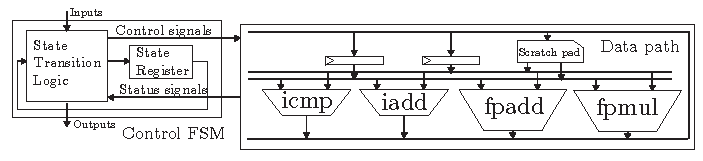
\includegraphics[width=3.5in]{./imgs/singleHLSArch_v2.pdf}
%\caption{Diagram representing a HLS circuit for the Matrix Multiplication example}
%\label{fig:singleHLSArch}
%\end{figure}


\begin{figure}[t]
\begin{lstlisting}[label={lst:MMM}, captionpos=b, caption={Matrix Multiplication Example}]
void MMM(float A[5][5],float B[5][5],float C[5][5])
{ int i=0, j=0, k=0;
  for(i=0, i<5, i++){
    for(j=0, j<5; j++){
      C[i][j] = 0;
      for(k=0, k<5; k++){
        C[i][j] += A[i][k]*B[k][j]; }
    }
  }
}
\end{lstlisting}
\vspace{-7mm}
\end{figure}

Figure \ref{fig:singleHLSArch} provides a diagram of the HLS generated
circuit for our matrix multiplication example.
Two clear partitions can be seen, a data path where functional units reside, and a
control FSM responsible for scheduling instructions onto the functional units.
In order to replicate only the control-flow structure
any data-path functional units which may influence a state transition need to be
duplicated along with the control FSM.

Analysing the code in Listing \ref{lst:MMM} we can determine that the instructions
which influence control-flow decisions are the ones used in the \lstinline{for} loop
conditions, which require an integer comparator \textbf{icmp} and adder \textbf{iadd}.
While the expensive floating point units, \textbf{fpmul} and \textbf{fpadd}, required
for calculating the inner dot product on line 7 have no
influence over any branch decision and will not be replicated.

Manually inspecting code and removing elements that don't influence control flow
may be feasible in the simple case of Matrix Multiplication, however as the complexity of the input increases
the engineering effort required in both analysing the input source and a generating circuit with an identical control FSM is
significant.
StitchUp fully automates this process through using a static analysis technique, known as program slicing, to extract
and duplicate any instructions that may influence control. The contribution of this paper are:

\vspace{-4pt}
\begin{itemize}
	\setlength{\itemsep}{1pt}
	\setlength{\parskip}{0pt}
	\setlength{\parsep}{0pt}
	\item StitchUp, a tool which can automatically extract and protect the control flow structure of a circuit generated with a HLS tool.
	\item Detailed results of StitchUp on the CHStone benchmark, where exhaustive hardware fault injection is performed on the majority of cases.
	\item Results exploring the reliability of StitchUp protected circuits as the control to data ratio is varied through
	loop unrolling in the matrix multiplication example.
\end{itemize}
%\vspace{1mm}
%\noindent
%$\bullet$ StitchUp, a tool which can automatically extract and protect the control flow structure of a circuit generated with a HLS tool.
%
%\vspace{1mm}
%\noindent
%$\bullet$ Detailed results of StitchUp on the CHStone benchmark, where exhaustive hardware fault injection is performed on the majority of cases.
%
%\vspace{1mm}
%\noindent
%$\bullet$ Results exploring the reliability of StitchUp protected circuits as the control to data ratio is varied through loop unrolling in the matrix multiplication example.


\section{FPGA device faults due to soft-errors}
\begin{figure}[t]
\centering
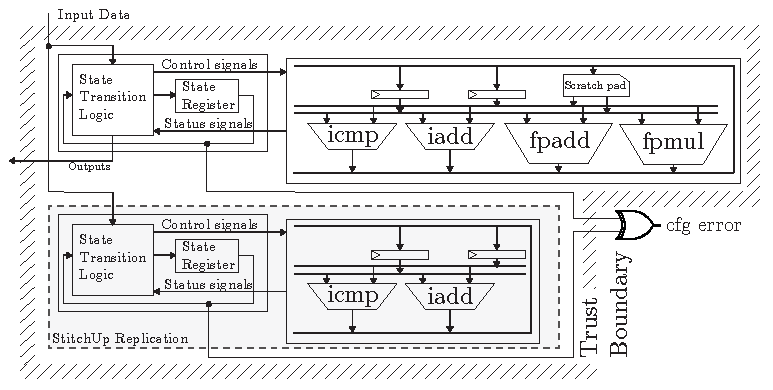
\includegraphics[width=3.5in]{./imgs/StitchUpReplication.pdf}
\caption{Default circuit (a) and Control Replicant (b) for our Dot Product example in Listing \ref{lst:DotProduct}, with Trust Boundary \vspace{-5mm}}
\label{fig:HLSArch}
\end{figure}

A Soft Error or Single Event Upset is a random, non-catastrophic error, where radiation causes
a perturbation to a circuit by temporarily altering a single signal or datum.
Detecting and mitigating such errors is important in some fields, such as satellite design,
where high design costs, \textbf{harsh environments}, and the difficulties in repairing once deployed make it necessary.
Additionally, due to the continuing increase in semiconductor density, the current soft error challenges 
experienced in space will also occur in future terrestrial devices.\cite{normand1996single}\cite{henkel2013reliable}.

FPGA devices work by mapping circuit descriptions into a collection of Logic Elements,
which are described in programmable Look-Up-Tables (LUTs) and routed together via
programmable switchboxes.
Configuration data for both the look-up-tables and switchboxes are stored in an SRAM based
configuration memory, which means soft errors can either change the functionality
of Logic Elements or can change the routing between them.
Other memories called block memory and flip-flops are also present in FPGA devices,
and soft errors in these regions can cause transient errors in the circuit.

%How this changes the protection strategy compared to software and VLSI
For ASIC designs, registers are the most vulnerable to soft-errors with
combinational logic contributing very little to overall circuit relability \cite{baumann2005soft}.
This makes ASIC approaches which analyses and protect vulnerable registers, such as in \cite{chen2014reliability},
promising approaches.
However in FPGA devices the most vulnerable region is the SRAM based configuration memory,
so such approaches would have little impact requiring methods perform combinatorial logic
replication such as StitchUp or DMR/TMR.

%ECC and frame based checking approaches
Circuits described within configuration memory are usually protected in one of two ways:
(1)the circuit is replicated with comparison; (2)ECC/CRC signals associated with
frames of the configuration memory are regularly scanned for errors.
Replication uses extra area and power but has low error detection latency and can
protect both configuration memory and registers,
while ECC/CRC checks consume less area and power in exchange for higher detection 
latency and an inability to protect registers.

For this paper our \emph{fault model} assumes that a single soft error
can occur at most every clock cycle, and that this error can effect block memory,
SRAM configuration memory, or flip-flops.
Since errors are not solely within the configuration memory, replication must be used,
as configuration ECC/CRC cannot protect the registers in our control structure.
Figure \ref{fig:HLSArch} shows a StitchUp generated circuit for the dot product 
example in Listing \ref{lst:DotProduct}, with the original circuit on top and the
control-flow structure shadow beneath it.
StitchUp aims to protect all configuration, block, and Flip-flop bits within the
trust boundary (grey box) as everything outside, such as routing to
external I/O or DDR, is not protected.



\section{StitchUp Overview} %Talk generally about the tool and what we are aiming to protect (Formal stuff goes here)
Finding and extracting the high-level control-flow structure from an RTL description
of a large circuit is difficult, whether it is attempted automatically or manually.
Finding the high-level control-flow in a high-level input source is easy, but manually
extracting an equivalent circuit is still challenging for large designs.
StitchUp can automatically perform this extraction as a compiler pass, which can be
easily invoked by setting a compiler flag in the LegUp HLS tool.
This section discusses how our analysis is implemented in StitchUp enabling the automatic extraction of the
control-flow structure along with the generation of the control replicant.
An open source version of our tool described in this paper can be found at
\emph{https://github.com/STFleming/StitchUp}.

\begin{figure}[t]
\centering
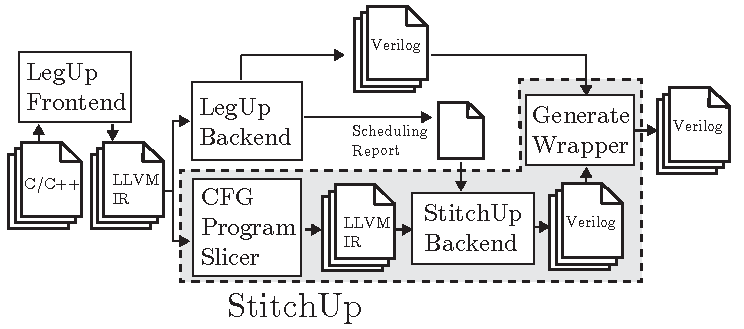
\includegraphics[width=3.5in]{./imgs/tool-flow.pdf}
\caption{Tool Flow Overview diagram}
\label{fig:tool_flow_diagram}
\end{figure}

%Flow Overview?
Figure \ref{fig:tool_flow_diagram} shows the transformation process from a C program
to a control-flow protected
Verilog hardware description, with StitchUp specific sections highlighted in grey.
Initially the C input is passed into the standard LegUp frontend, which is
a series of passes that
perform various tasks, such as annotating instructions with pipelining information.
This outputs an LLVM intermediate representation (LLVM-IR) which is passed both into the backend of LegUp,
to generate the
original unprotected circuit and also into the frontend of StitchUp to generate the control replicant circuit.
Finally an integration stage connects the original circuit to the duplicate control-flow circuit
and generates comparison logic to ensure that the state registers match.

%Why LegUp?
Our motivation for integrating our tool with LegUp is primarily due to it being open source, as
the StitchUp backend requires modification to the generation of the scheduling control FSMs.
However, the technique itself could be incorporated in VivadoHLS and all other HLS tools through modifying the
generated control FSM in a different fashion, (such as modifying the output HDL directly).
It is common for modern HLS tool to be constructed on top of LLVM-IR which has
a similar level of abstraction to assembly code.
It also has two important features for writing compiler optimisations:
first, all instructions are in single static assignment form (SSA) where every variable is only
assigned once; and second, instructions are grouped into straight-line sequences known as basic blocks (BB)
where there is only one entry branch at the very start of the block, and one exit branch at the very end.

\begin{figure}[t]
\centering
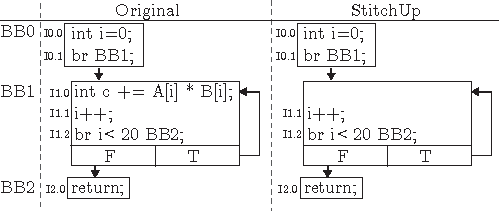
\includegraphics[width=3.5in]{./imgs/dot_product_cdfg.pdf}
\caption{Control-Data-Flow Diagram for Matrix Multiplication example}
\label{fig:mmm_cdfg}
\end{figure}

\subsection{Extracting the Control Instruction Set}
LLVM-IR, which is passed into the frontend of StitchUp, is naturally arranged into a CDFG
where each node is a basic block and edges are branch between them.
An example of the CDFG from the dot product in Listing \ref{lst:DotProduct}
is shown on the left side of Figure \ref{fig:mmm_cdfg}.
The StitchUp frontend performs a backwards analysis walking the CDFG from bottom to top, collecting any control flow
related instructions that may influence whether an edge transition is taken.

All instructions deemed to be control related are collected into what we refer to as a Control Structure Instruction Set ($\mathit{CSIS}$),
which can be used to generate a control replicant.
Each basic block, $i$, in the input CDFG will have it's own associated $\mathit{CSIS}_{i}$ containing all instructions that may effect
control-flow after this point in the program.
The overall $\mathit{CSIS}$ for the input is $\mathit{CSIS}_s$ where $s$ is the initial basic block of the input program.

Algorithm \ref{alg:CSIS-extraction} is used to construct the $\mathit{CSIS}$ for all nodes in the CDFG.
It requires a fixed point iteration until the set of all $\mathit{CSIS}$, $C_{\mathit{CSIS}}$ has reached a stable state
which can be seen in line 1-2.
Each iteration walks backwards from the final basic block of the CDFG to the start basic block, as seen in
line 3, and for each encountered the corresponding $\mathit{CSIS}$ is updated using the following rules:

%\vspace{-4pt}
\begin{enumerate}[label=Rule \arabic*]
    \setlength{\itemsep}{3pt}
    \setlength{\parskip}{0pt}
    \setlength{\parsep}{0pt}
    \item $\mathit{Sucessor(B)}$ returns the set of all basic blocks in the CDFG that follow on from the basic block $B$.
	  For all successor  $j$ of basic block $i$ this rule adds every element of $\mathit{CSIS}_j$ to $\mathit{CSIS}_i$.
    \item Adds all branch instructions for the current basic block, $i$, to $\mathit{CSIS}_i$ using
	  $\mathit{TerminatingInstruction(i)}$ a function which returns the final instruction from the basic block $i$.
    \item Any instruction within the current basic block ($i$) that is used as an operand ($\mathit{op_{c}}$) by an element of $\mathit{CSIS}_i$ is added to $\mathit{CSIS}_i$ \footnote{For the current version of the tools the worst case is assumed for memory operations.}
\end{enumerate}
\vspace{-4pt}

\begin{algorithm}[h]
\caption{$\mathit{CSIS}$ Extraction Static Analysis Algorithm
\label{alg:CSIS-extraction}}
    \begin{algorithmic}[1]
        \INPUT a program, $P$, set of Basic Blocks, \{$\mathit{BB}_0$...$\mathit{BB}_N$\}
        \OUTPUT $P'$ a program consisting of $I_c$ the set of control structure instructions.
        \Statex
        \While{$C_{\mathit{CSIS}}$ != $P_{\mathit{CSIS}}$}
            \State $P_{\mathit{CSIS}} \gets \{\mathit{CSIS}_{\mathit{BB0}}, \dots,  \mathit{CSIS}_{BBN}$\}
            \For{\textbf{each} $B \in \{BB_{N},\dots,BB_{0}\}$}
                \\\hrulefill
                \For{\textbf{each} $S \in Successor(B)$}\Comment{Rule 1}
                    \For{\textbf{each} $I_{c} \in \mathit{CSIS}_{S}$}
                        \State $\mathit{CSIS}_B \cup \{I_{c}\}$
                    \EndFor
                \EndFor
                \\\hrulefill

                \State $T \in TerminatingInstruction(B)$\Comment{Rule 2}
                \State $\mathit{CSIS}_{B} \cup \{T\}$
                \For{\textbf{each} $op \in T$}
                    \State $\mathit{CSIS}_{B} \cup \{op\}$
                \EndFor
                \\\hrulefill

                \For{\textbf{each} $I \in B$}\Comment{Rule 3}
                    \For{\textbf{each} $I_c \in \mathit{CSIS}_{B}$}
                        \For{\textbf{each} $op_c \in I_c$}
                            \If{$I = op_{c}$}
                                \State $\mathit{CSIS}_{B} \cup \{I\}$
                            \EndIf
                        \EndFor
                    \EndFor
                \EndFor
            \EndFor
	\State $P' \gets \mathit{CSIS}_{\mathit{BB0}}$
        \EndWhile
    \end{algorithmic}
\end{algorithm}

To demonstrate this we will apply Algorithm \ref{alg:CSIS-extraction} to the
dot product example in Listing \ref{lst:DotProduct} to extract the control-flow structure, 
labelled StitchUp in Figure \ref{fig:mmm_cdfg}. 
For each update to a $\mathit{CSIS}$, the label for the instruction added from \ref{fig:mmm_cdfg} is given 
along with the rule from Algorithm \ref{alg:CSIS-extraction} used to add it. 

%-------------------------------------------------------
\vspace{1mm}
\noindent
\textbf{Initially} $\mathit{CSIS}_{i} = \emptyset$ for all basic blocks $i$

\vspace{-2mm}
\noindent
\hrulefill

\vspace{-1mm}
\noindent
\textbf{Iteration 1:}

%----BB2----
\FirstAnalysisTraceRule{BB2}{I2.0:\textbf{return}}{2}
\CSISState{BB2}{I2.0}
%----BB1----
\FirstAnalysisTraceRule{BB1}{every element in $\mathit{CSIS}_{BB2}$}{1}
\AnalysisTraceRule{I1.2:\textbf{br i<20 BB2}}{2}
\AnalysisTraceRule{I1.1:\textbf{i++}}{3}
\CSISState{BB1}{I2.0,I1.2,I1.1}
%----\mathit{BB0}----
\FirstAnalysisTraceRule{\mathit{BB0}}{every element in $\mathit{CSIS}_{BB1}$}{1}
\AnalysisTraceRule{I0.1:\textbf{br BB1}}{2}
\AnalysisTraceRule{I0.0:\textbf{i=0}}{3}
\CSISState{\mathit{BB0}}{I2.0,I1.2,I1.1,I0.1,I0.0}

\vspace{1mm}
\noindent
\textbf{Iteration 2:}\hspace{3mm} No Change, fixed point reached
%-----------------------------------------------------

\vspace{1mm}

Once the analysis is completed the final value of $\mathit{CSIS}_{\mathit{BB0}}$ is turned into LLVM-IR
and given to the StitchUp backend.
Here scheduling information from the original unmodified LegUp flow is used to generate
an identical control FSM to the original circuit, often requirng the insertion of blank states
used to schedule instructions that have not been included in the control replicant. 
Finally, an integration stage takes the original LegUp and StitchUp circuits,
adds comparison logic to compare the state registers of the two circuits in each cycle,
and generates a top level wrapper to connect them


\section{Experiment Setup}
\begin{figure*}[t]
\centering
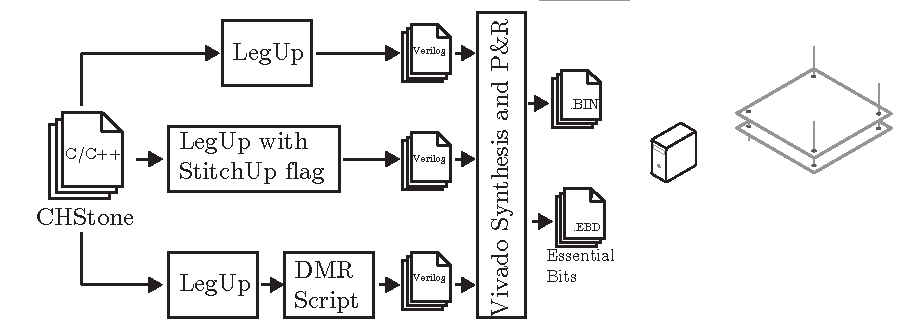
\includegraphics[width=6in]{./imgs/ExperimentFlow.pdf}
\caption{The experiment flow}
\label{fig:ExperimentFlow}
\end{figure*}

To test the error mitigation abilities of StitchUp generated circuits we have adopting the
gold standard of hardware fault injection, where configuration bits on the 
FPGA device are flipped from their original state.
Typical FPGA designs will require a large number of configuration bits often making
full exhaustive testing infeasible, usually resulting in the adoption of random
testing.
However in our case we have developed an experiment
platform allowing us to achieve full exhaustive fault injection in reasonable time,
for example reducing the time to exhaustively test the smallest CHStone circuit dfmul from 4 days
to 8 hours.

We make use of many low cost Xilinx FPGA SoC devices known as
Zedboards all injecting on the same circuit in parallel.
Each Zedboard runs a full Linux OS on its hardened ARM processor, and is arranged into
a cluster managed by a single desktop\footnote{Called The SoC Drawer}.

To flip individual configuration bits a Xilinx Soft Error Mitigation (SEM) IP Core
connected to the FPGA internal configuration port (ICAP) was used --
targeting Xilinx devices was possible due to the latest release of LegUp
(v4.0) which has the ability to generate generic Verilog circuits.
For each experiment the SEM core and the test circuit were instantiated and connected to the
ARM processing system via AXI interconnects.
%Software running under Linux on each ARM core managed each test by first sending an error
%address and injection command to the SEM core, then starting the circuit under test,
%and finally collecting the error (if any) associated with that address.

Figure \ref{fig:ExperimentFlow} shows an overview of the experiment setup.
The top flow generates a standard LegUp circuit with no protection;
the middle uses StitchUp to generate a control-flow structure protected circuit;
and the bottom generates a full DMR protected circuit duplicating the original LegUp
circuit and generating comparison logic on the control FSM state register;

Each different version is then passed through the Xilinx FPGA circuit tool flow to produce
two files: an essential bits file (.EBD), and a configuration binary (.BIN).
The essential bits file is a list of configuration memory bits that have any
influence on our generated circuit and is used to reduce the number of injections
required to fully test our design.\footnote{Essential bits do not contain BRAM data,
since these are considered transient data not essential}
For each experiment the EBD files are divided up into smaller chunks, and each chunk is
processed in parallel on a different Zedboard device.

Software running on the ARM of each Zedboard marshals each test by, injecting a fault,
running the circuit, and storing the result.
The injected fault is then repaired by re-injecting an error into the
same configuration memory location (i.e. flipping the bit back to it's original state).
Some faults may cause the circuit to never terminate, so if no response is seen within three orders
of magnitude of its expected time a, timeout halts its execution.

The results are then analysed and each test outcome is classified into three distinct categories:

\begin{enumerate}
\setlength{\itemsep}{1pt}
\setlength{\parskip}{0pt}
\setlength{\parsep}{0pt}
\item Execution Time Error \textbf{ETE} - This is where the execution of the circuit either took
an incorrect number of cycles to complete or timed out. Errors of these type are
control flow related, since any deviation from the correct execution path will cause
an incorrect number of cycles.
\item Data-Flow Only Errors \textbf{DOE} - These are errors where the circuit has returned an incorrect
data result but has executed in the correct number of cycles, such as error caused
by faults in a non-control structure functional unit.
\item Caught Errors \textbf{CE} - These are errors in the state register that were detected by the protection method, which is
either DMR or StitchUp.
\end{enumerate}

For each test the proportion of ETE, DOE, and CE error results should sum to 100\%.
ETEs are the most critical since they are control related and may runtime guarantees and timeouts;
DOEs are the next critical category since there is an error in data, but no damaging effect on control;
and CEs are the least critical, where the circuit has failed but at least it has been detected.


\section{Experiment Results}
\subsection{Resource Results}
\begin{table*}[t]
\small
\singlespace
\centering
\caption{Resource Usage Results}
\label{tab:resources}
\tabcolsep=0.11cm
\begin{tabular}{@{}|l|l|l|l|l|l|l|l|l|l|l|l|l|@{}}
\toprule
                    & \multicolumn{4}{l|}{\textbf{Original}}                      & \multicolumn{4}{l|}{\textbf{StitchUp}}                      & \multicolumn{4}{l|}{\textbf{DMR}}                           \\ \midrule
\textbf{Benchmarks} & \textit{LUT} & \textit{REG} & \textit{DSP} & \textit{Power} & \textit{LUT} & \textit{REG} & \textit{DSP} & \textit{Power} & \textit{LUT} & \textit{REG} & \textit{DSP} & \textit{Power} \\ \midrule
\textit{aes}        & 47230        & 28152        & 0            &                & 47539        & 28800        & 0            &                &              &              &              &                \\ \midrule
\textit{adpcm}      & 21050        & 16752        & 168          &                & 29599        & 29484        & 178          &                &              &              &              &                \\ \midrule
\textit{blowfish}   &              &              &              &                &              &              &              &                &              &              &              &                \\ \midrule
\textit{dfadd}      & 4639         & 4310         & 0            &                & 5562         & 5095         & 0            &                & 6394         & 5754         & 0            &                \\ \midrule
\textit{dfdiv}      & 12144        & 13157        & 30           &                & 22254        & 23449        & 60           &                & 22811        & 23904        & 60           &                \\ \midrule
\textit{dfmul}      & 3348         & 3912         & 16           &                & 4553         & 4845         & 32           &                & 5105         & 5397         & 32           &                \\ \midrule
\textit{dfsin}      & 21343        & 20347        & 71           &                & 40928        & 38116        & 136          &                &              &              &              &                \\ \midrule
\textit{gsm}        &              &              &              &                &              &              &              &                &              &              &              &                \\ \midrule
\textit{jpeg}       &              &              &              &                &              &              &              &                &              &              &              &                \\ \midrule
\textit{mips}       & 8278         & 6367         & 4            &                & 15639        & 10231        & 8            &                & 14304        & 10351        & 8            &                \\ \midrule
\textit{motion}     &              &              &              &                &              &              &              &                &              &              &              &                \\ \midrule
\textit{sha}        & 9117         & 9287         & 3            &                & 9491         & 10188        & 6            &                & 16788        & 16189        & 6            &                \\ \bottomrule
\end{tabular}
\end{table*}


\begin{figure}[h]
\centering
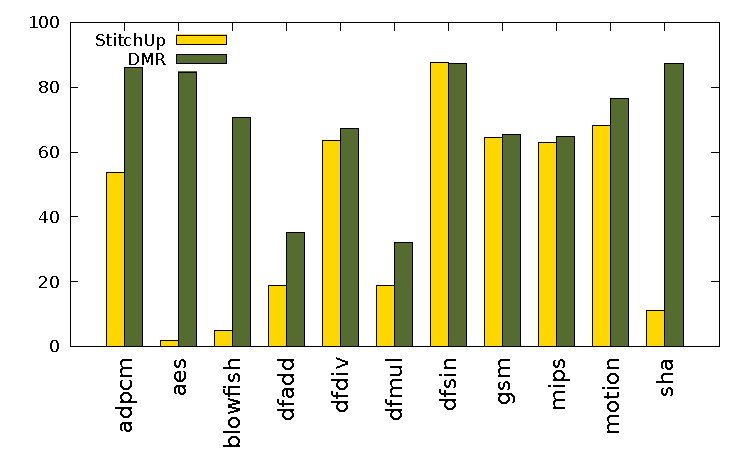
\includegraphics[width=2.5in]{./graphs/chstone_luts_24_09_2015.pdf}
\caption{Luts for the CHStone benchmark}
\label{fig:luts_result}
\end{figure}

\begin{figure}[h]
\centering
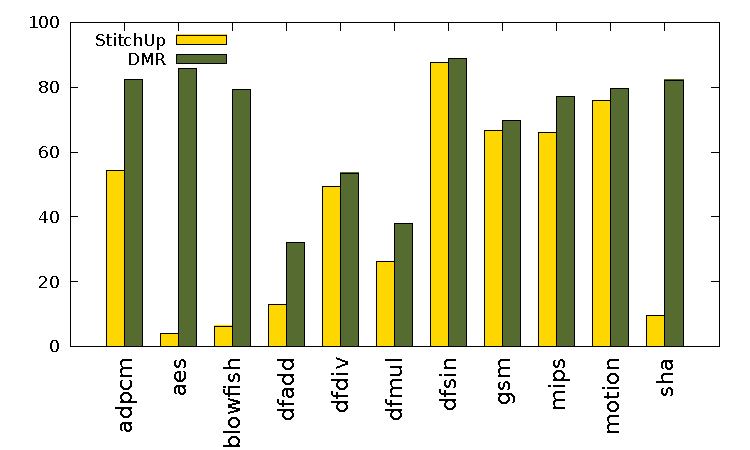
\includegraphics[width=2.5in]{./graphs/chstone_reg_24_09_2015.pdf}
\caption{REGs for the CHStone benchmark}
\label{fig:regs_result}
\end{figure}

\subsection{Power Results}

\begin{figure}[h]
\centering
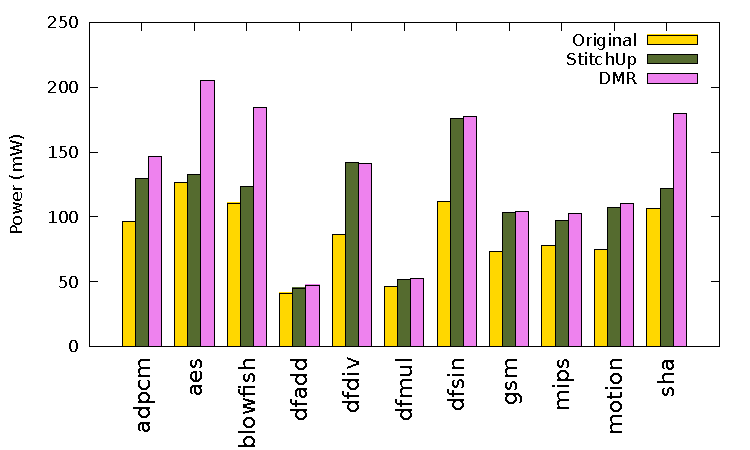
\includegraphics[width=2.5in]{./graphs/chstone_absolute_power_24_09_2015.pdf}
\caption{Power for the CHStone benchmark}
\label{fig:power_result}
\end{figure}

\subsection{Fault Injection Results}


\section{Related Work}
%RELATED WORK SECTION
%Intro to HLS approaches
Early work such as \cite{antola1998high} examined how hardware redundancy 
could be reduced when using HLS to generate DMR circuits.
The authors present a scheduling and alloction algorithm, where the circuit duplication is optimised
so that idle resources are reused instead of instantiating multiple hardware copies.
They manage to successfully reduce the area requirments, while avoiding error aliasing.

%Libary based approaches for Allocation stage of HLS tools
More recent work has instead of using redundancy examined how reliability can be optimised by 
selecting different implementations of components during allocation.
In \cite{tosun2005reliability}
a library of components annotated with area, power, and reliability metrics is used during component selection.    
Initially the set of most reliable components is selected, and then itterative optimisation passes attempt to
meet constraints on the other metrics in a fashion similar to power-aware HLS approaches. 

In \cite{glass2007interactive} this library approach is extended to include the replication of some components 
and an evolutionary algorithm is used to present the results to the user as a design space exploration.
As work in \cite{hara2013cost} extends it to encorporate reliability decisions into scheduling, arguing that
the longer a functional unit is active the more likely it will experience a fault. 

%Application level protection, what can we skip?
The methods discussed so far all propose changes to the underlying HLS algorithms,
none of them  investigate how the input source can be analysed beforehand to extract
critical and non-critical sections of code.
But do such critical and non-critical sections exist?

%HLS methods that exploit the static analysis of input code
Other recent work includes \cite{chen2014reliability} where the vulnerability of variables is analysed and the most vulnerable
variables for a HLS program are protected by assigning them to special registers.
The proposed variable vulnerability analysis takes into account their lifetimes, dependencies, and branch probabilities.
Through analysing the CDFG, error and branch probabilities are used to propagate error likelihood forward to estimate the total
vulnerability for each variable in the design.
A Integer Linear Program solver is then used to minimise the subset of protected registers to cover the maximum number of variables.
They build their results on top of LegUp, and use LLVM to perform the variable vulnerability analysis.
They achieve impressive results, where protecting 20\% of the registers results in more than 60\% soft error mitigation in the best case.
However full fault injection tests are not performed on the generated hardware, and only state-based probabilistic error testing
was performed.\\

%What we are aiming to do differently.


\section{Conclusion}
Control-flow errors can be catastrophic, causing real-time deadlines to be missed, or worse non-termination.
This work presents StitchUp a compiler flag for the Open Source HLS tool LegUp, which can automatically extract and protect the control-flow of an input program.
To demonstrate this we applied it to the popular HLS benchmark suite CHStone and performed exhaustive hardware error injection on a selection of circuits.
Our results show that StitchUp is capable of detecting all execution time errors while requiring a smaller fraction of the resources and power than DMR.


% The following two commands are all you need in the
% initial runs of your .tex file to
% produce the bibliography for the citations in your paper.
\bibliographystyle{abbrv}
{\small \bibliography{refs}}  % sigproc.bib is the name of the Bibliography in this case
% You must have a proper ".bib" file
%  and remember to run:
% latex bibtex latex latex
% to resolve all references
%
% ACM needs 'a single self-contained file'!
%
%APPENDICES are optional
%\balancecolumns
%\appendix
\end{document}
